%!TEX root = ../thesis.tex

\chapter{2D Heat Transfer Methodology}

This chapter showcases one of the simplest heat transfer cases, which is a brick wall heat transfer methodology.
Understanding what resources and capabilities can be utilized from hand calculation until digital simulation is a necessity to move to 3D in the next chapter. Thus, this chapter presents different approaches to finding the 2D brick wall heat flux. First, an estimation of the heat flux was calculated manually. Then, the same boundary conditions were used in an experimental design, resulting in the same heat flux value. Followed by, implementing the same brick wall geometry, boundary conditions, and materials in HTflux which is a 2D heat transfer software and the resulting heat flux complies with the previous results as well. %dont know if I should add this sentence below
Finally, this 2D brick wall will be implemented in the \gls{OF} 3D heat transfer tool presented in this project to see if the temperatures and heat flux comply with the results from the previous approaches. 




\section{Manual Estimation of Heat Flux}
This section presents the simplest heat flux calculation that can be performed manually. This exercise is the first and most traditional approach to finding heat flux for a simple brick wall geometry. The heat flux calculation for the 2D section shown in \ref{fig:2d2} \textbf{(a)} is as follows:
\begin{equation}
q = -k \frac{dT}{dx}
\end{equation}

where q is the heat flux,
k is the Thermal conductivity, and
$\frac{dT}{dx}$ is the Temperature gradient, which can be found by $\frac{T_2 - T_1}{L}$ over thickness L \cite{heattransfund}. 

Solving for q where k = 1 ${W/m}^2$, 
L = 0.43 m,
$T_1$ = 25.8 \, $^\circ$ \text{C}, 
$T_2$  = 21.1 \, $^\circ$ \text{C}



Substituting the given values:
\[ q = -1 \, \text{W/m}^2 \times \frac{21.1 \, ^\circ \text{C} - 25.8 \, ^\circ \text{C}}{0.43 \, \text{m}} \]
\[ q = 10.93 \, \text{W/m}^2 \]
So, the heat flux \( q \) is \( 10.93 \, \text{W/m}^2 \).





\section{Heat Flux Sensors Experiment}



This section presents the second approach to find heat flux, which is a real-time measurement of the 2D brick wall. The experiment was carried out in 358D office located in the Hinman Research building with a duration of 74 hours using U-value and heat flux sensors as shown in \ref{fig:figexp1} \textbf{(a)} and \ref{fig:figexp1} \textbf{(b)}. The experiment started on March 14th, 2024 at 14:24:15 until March 17th, 2024 at 15:24:15. 
The experimental design details and results are showcased in the upcoming subsections.


\begin{figure}[htb]
    \centering
    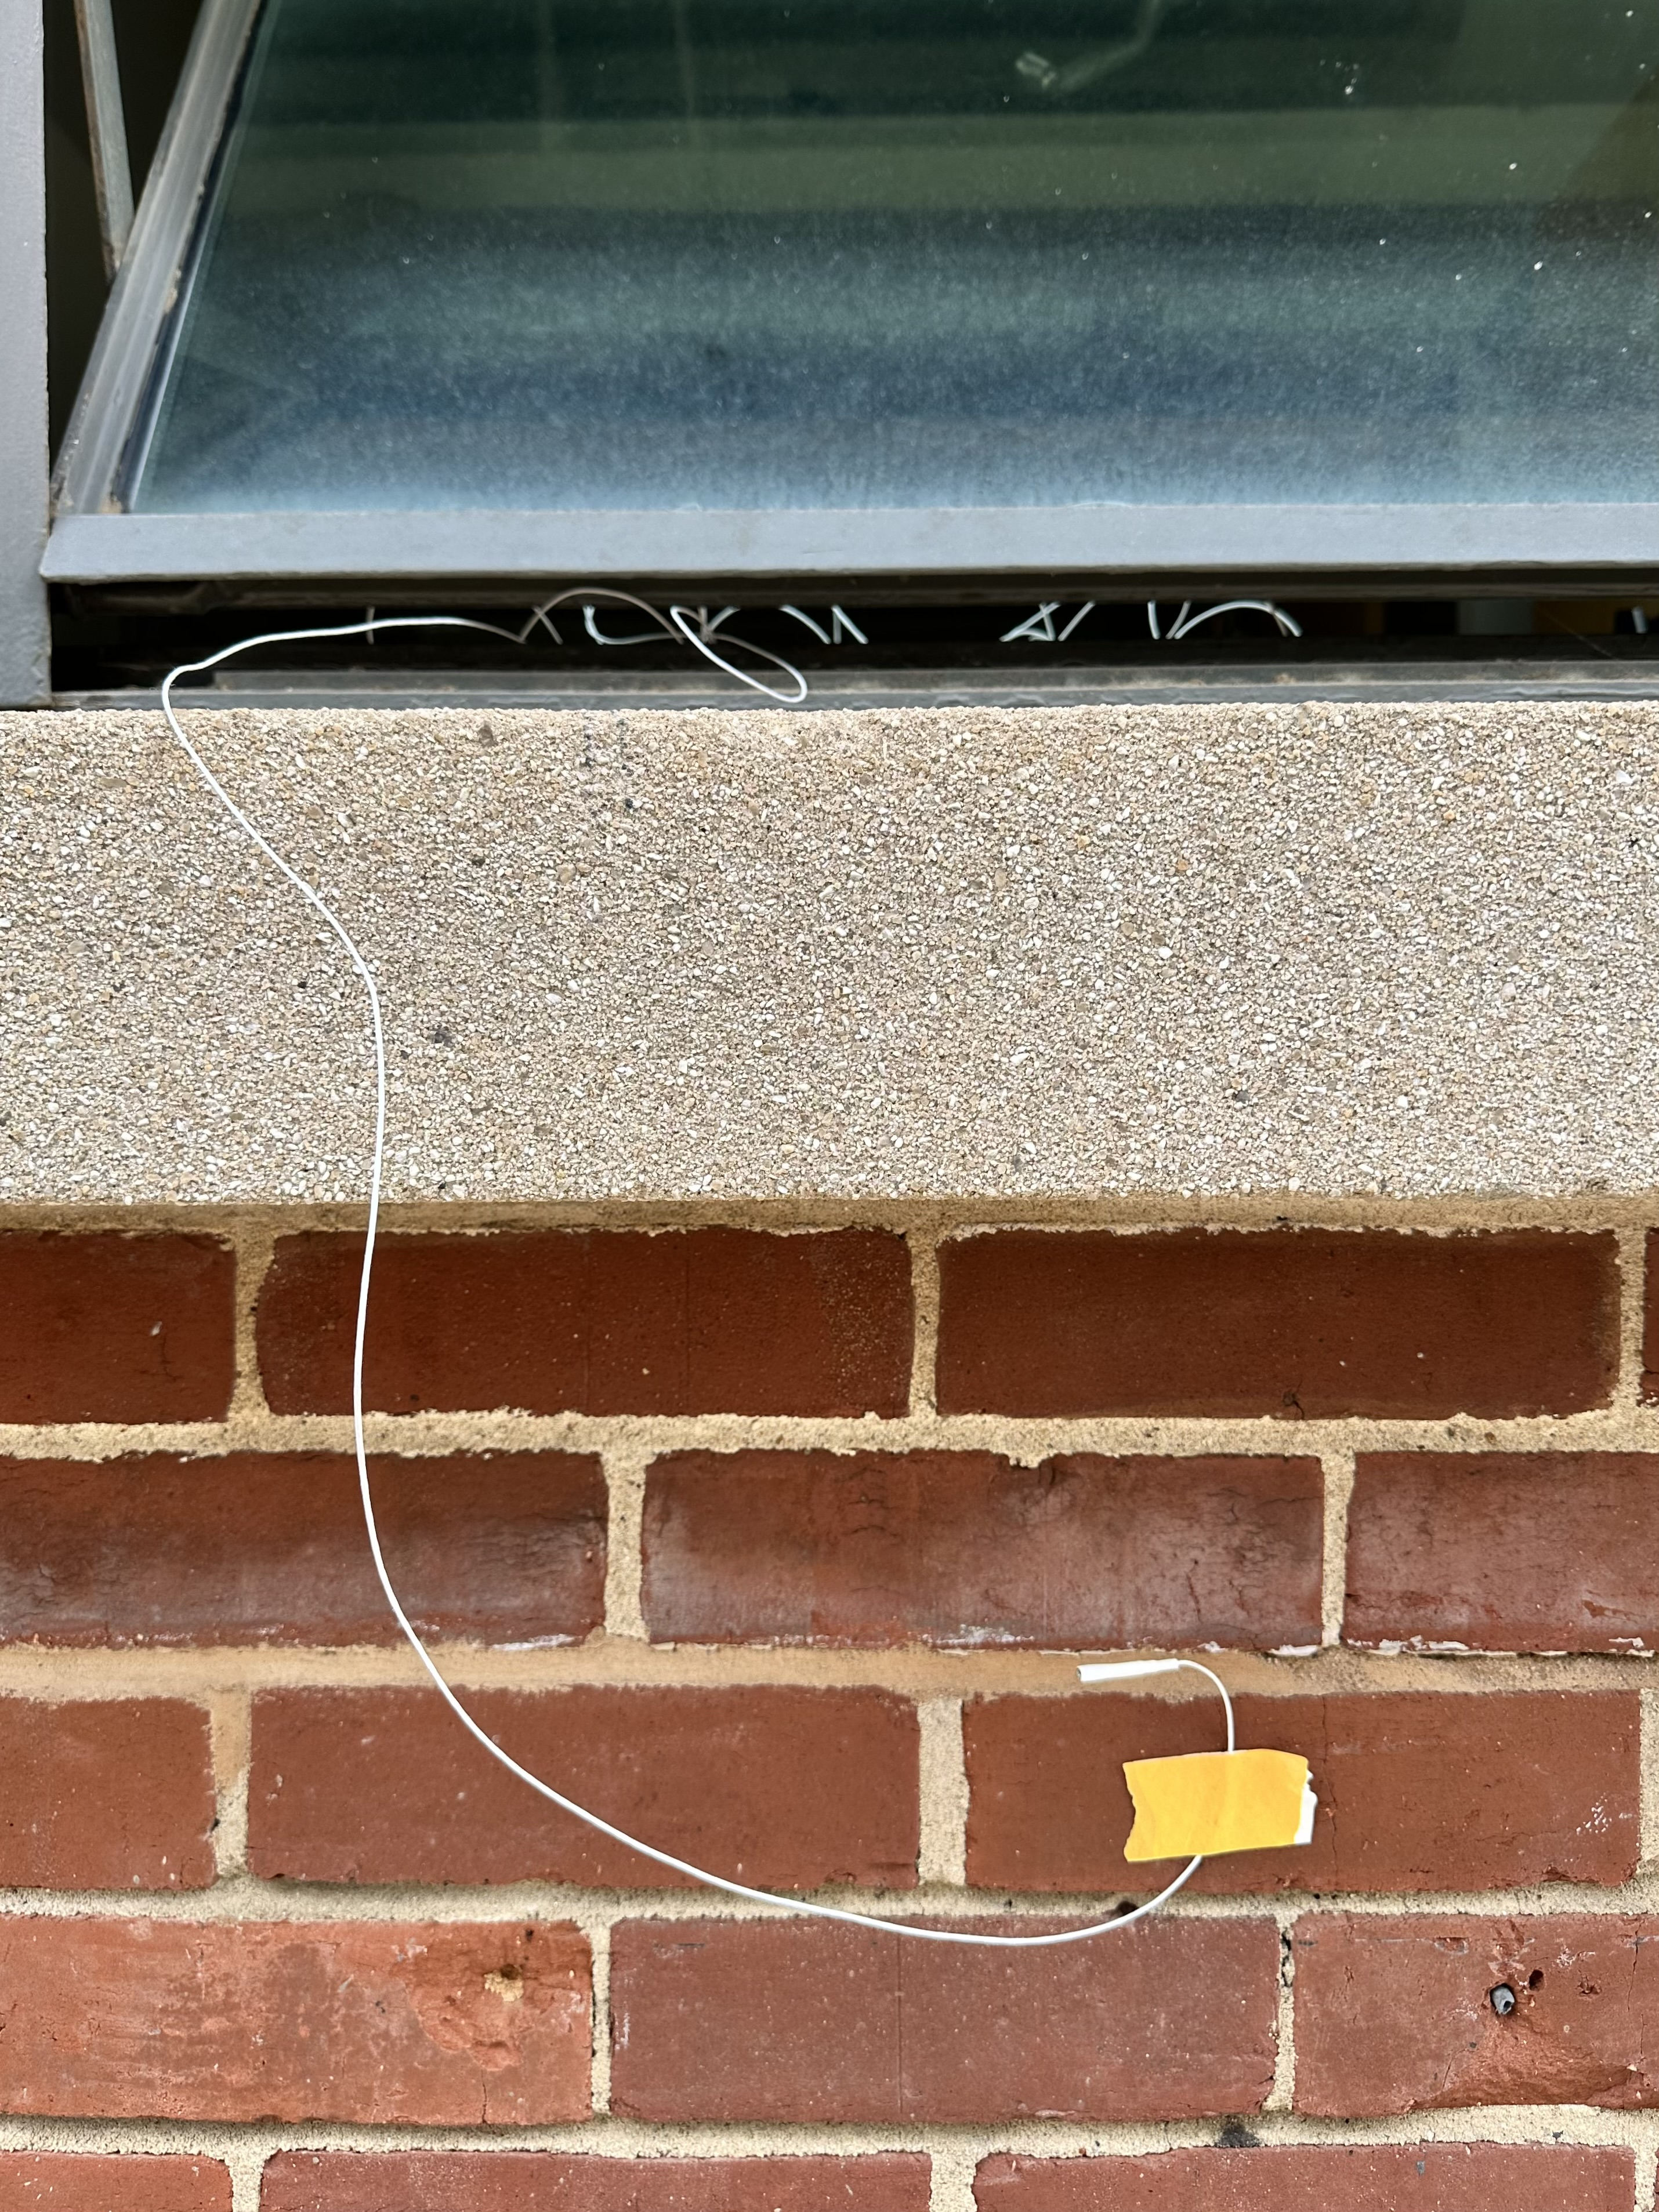
\includegraphics[width=0.495\linewidth]{Figures/expfig1.jpg}
    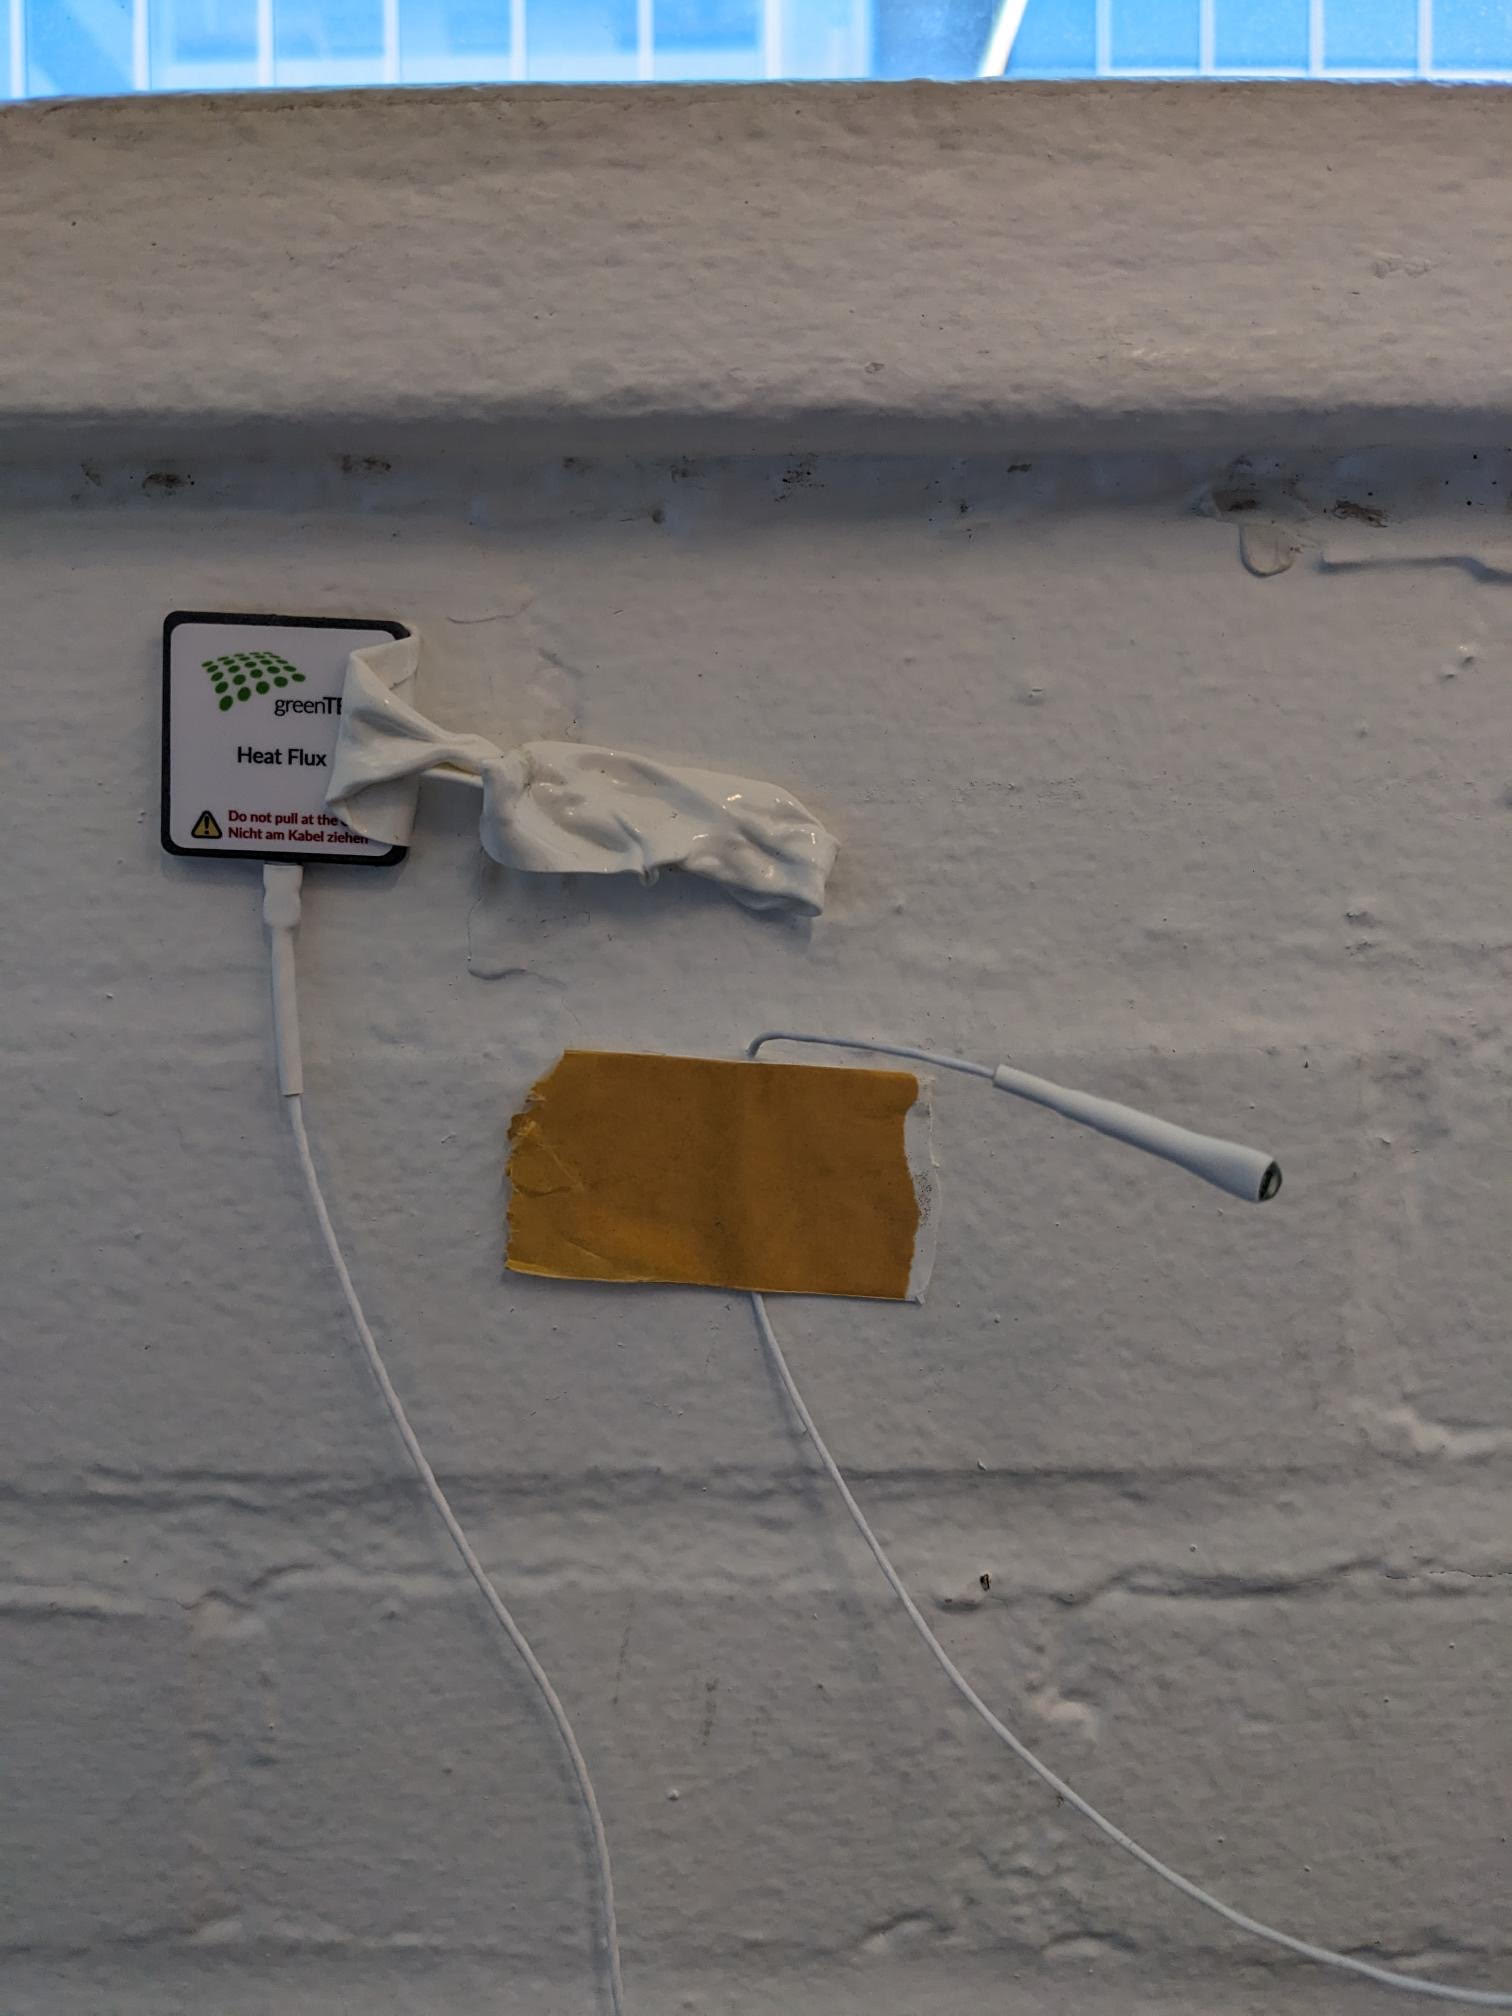
\includegraphics[width=0.495\linewidth]{Figures/expfig2.jpg}

    \hspace{3.5cm}\textbf{(a)}\hfill\textbf{(b)}\hspace{3.7cm}

     \caption[Experimental heat flux measurement setup]{Outdoor heat flux sensors during experimental design. The window was closed as much as possible to avoid interference with the sensor cord \textbf{(a)}. Indoor heat flux sensors during the experimental design \textbf{(b)}.}
   \label{fig:figexp1}
 \end{figure}




 
\subsubsection{Experimental Design}
 This experiment is based on using the measurement device used was the gSKIN® KIT-2615C (calibrated) U-Value and Heat Flux Measurement Kit from GreenTeg  \cite{greenteg} shown in \ref{fig:toolkit} and purchased by the funding received from Micro Research Grants for Regenerative Built Environments by  Kendeda Building Advisory Board \cite{kendeda}.
 \todo{fix this sentence}
 The schematic in \cref{fig:2d2} shows the experimental design setup with the same conditions of k  = 1 ${W/m}^2$ 
L  = 0.43 m,
$T_1$ = 25.8 $^\circ \text{C}$, 
$T_2$  = 21.1  $^\circ \text{C}$ .

\begin{figure}[tbh]
     \centering
    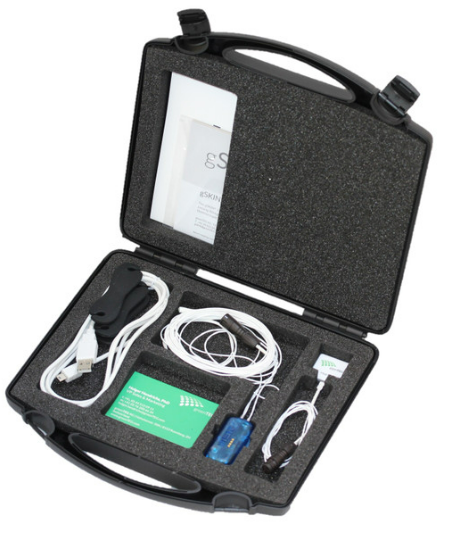
\includegraphics[width=0.5\linewidth]{Figures/greenteg.png}
     \caption[U-value measurement Kit]{The U-Value and Heat Flux Measurement Kit, for details see \cref{tab:u-value-measurement-kit}.}
   \label{fig:toolkit}
 \end{figure}






\subsubsection{Experiment Results}
This section showcases the results from sensor reading for the brick wall. The GreenTeg sensor company provides software to log and visualize the data, along with writing a final report with a CSV file documenting the reading on 10-second intervals. The chart in \ref{fig:expr} represents the temperature and heat flux results of the brick wall. 
The report indicates that the final resulting U value = 2.31 ${W/m^2k}$. Thus, according to the boundary conditions and the given results, the heat flux is \( q \) is \( 10.93 \, {W/m}^2 \). 
Where U-value from the report = 2.31 ${W/m^2k}$ and 
\begin{equation}
    U = \frac{k}{\text{L}}
      = \frac{1}{\text{0.43}} = 2.33  {W/m^2k}
\end{equation}
Where k = 1 \text{ W/(m²)}, L (thickness) = 0.43. So, \(U_{\text{calc}}\) = \(U_{\text{exp}}\) = 2.31 ${W/m^2k}$ 

\ref{fig:expr} below is a plot report showing the experimental design results of the fluctuations in indoor and outdoor temperature along with the heat flux. From the report, three temperatures from different time steps were selected to be compared with the 3D simulation results. Also, \ref{table2d} shows the comparison of the selected three points, where $T_{val}$ is the experiment's resulting temperature and $T_{sim}$ is the simulation's resulting temperature. 
The measurement approach represented in this section offers detailed time step values for temperature and heat flux. However, the cost of the sensor kit is considered high = \$2,157. Another issue with this approach is the time spent setting up and receiving results, where the minimum required reading time is 73 hours. Thus, the next section showcases an easier and faster method to find the heat flux, which using a 2D heat transfer simulation.

\begin{figure}[htb]
     \centering
    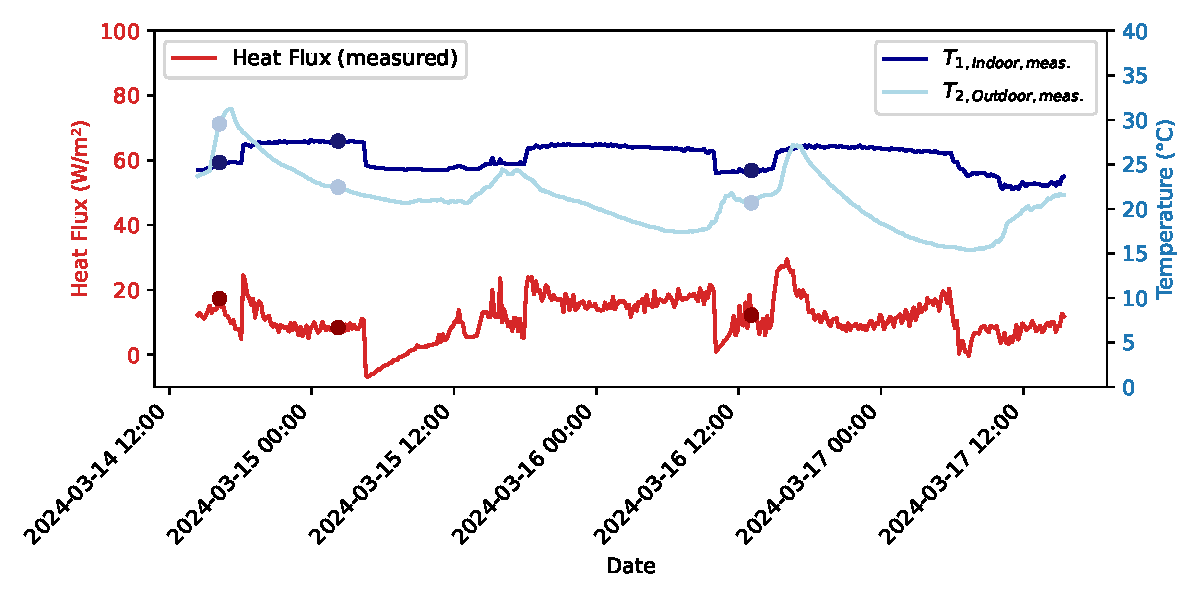
\includegraphics[width=1\linewidth]{Figures/Validation}
     \caption[2D Experimental Report Plot]{The line plots represent the sensor's heat flux and Temperature readings. where the points are the \gls{OF} simulation results.}
   \label{fig:expr}
 \end{figure}


\begin{table}[tbh]
    \caption{2D Temperature and Heat Flux Comparison}
    \label{table2d}
    \centering
    \begin{tabular}{lrrrrrrr}
        \toprule
        Time                & $T_{1,val,in}$ & $T_{1,sim,in}$ & $T_{2,val,out}$& $T_{2,sim,out}$ & $Q_{val}$ & $Q_{sim}$ \\
        \midrule
        3/14/2024 16:14 & 298.3    & 298.3    & 302.7     & 302.7     & 17.3 & 17.2 \\
        3/15/2024 02:14  & 300.7    & 300.7   & 295.5    & 295.6     & 8.9  & 8.3  \\
        3/16/2024 13:04 & 297.4  & 297.4   & 293.8   & 293.8   & 12.54 & 12.2  \\
        \bottomrule
    \end{tabular}
   
\end{table}




\begin{figure}[H]
  \centering
  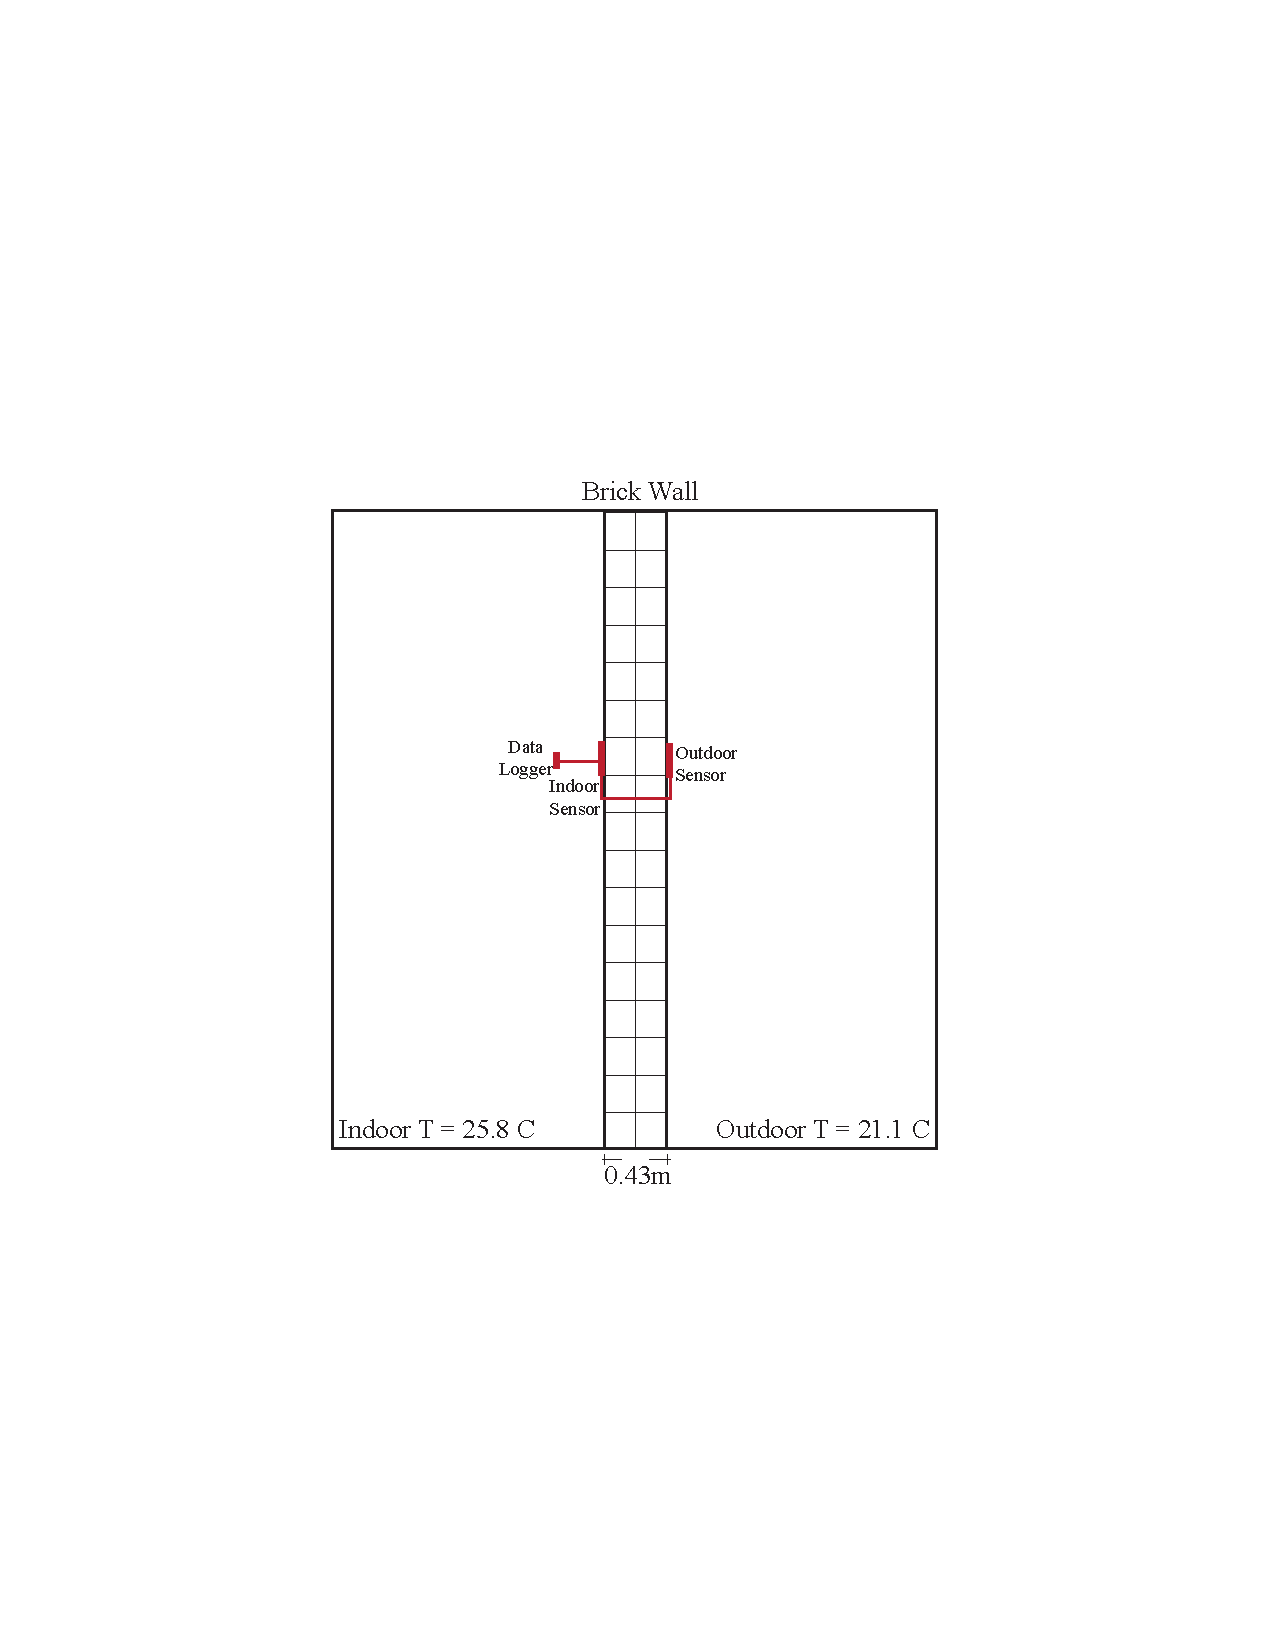
\includegraphics[trim=5.6cm 7.5cm 5.3cm 8cm, clip, width=.6\linewidth]{Figures/2dsection2.pdf}
\caption[2D Section and Setup]{Experiment setup for the 2D brick wall.}
\label{fig:2d2}
\end{figure}




















\section{Simulation}
\subsubsection{2D Simulation}
Moving to the third approach, which is using a 2D heat transfer software, where the same brick wall is modeled in HTFlux. HTFlux is a software that simulates 2D heat transfer seamlessly and calculates the heat flux with providing the temperature gradient \cite{HTflux}. The boundary conditions assigned in this simulation are the same as the previous methods which are ; brick thermal conductivity is k  = 1 ${W/m}^2$ 
L  = 0.43 m,
$T_1$ = 25.8 $^\circ \text{C}$, 
$T_2$  = 21.1  $^\circ \text{C}$ .


 \ref{2dconst} \textbf{(a)} which shows the materials and the boundary condition implemented in the software and \textbf{(b)} represents the 2D simulation results where the resulting heat flux = \( q \) is \( 10.91 \, {W/m}^2 \) as expected.










\begin{figure}[H]
\begin{minipage}{0.45\textwidth}
  \centering
  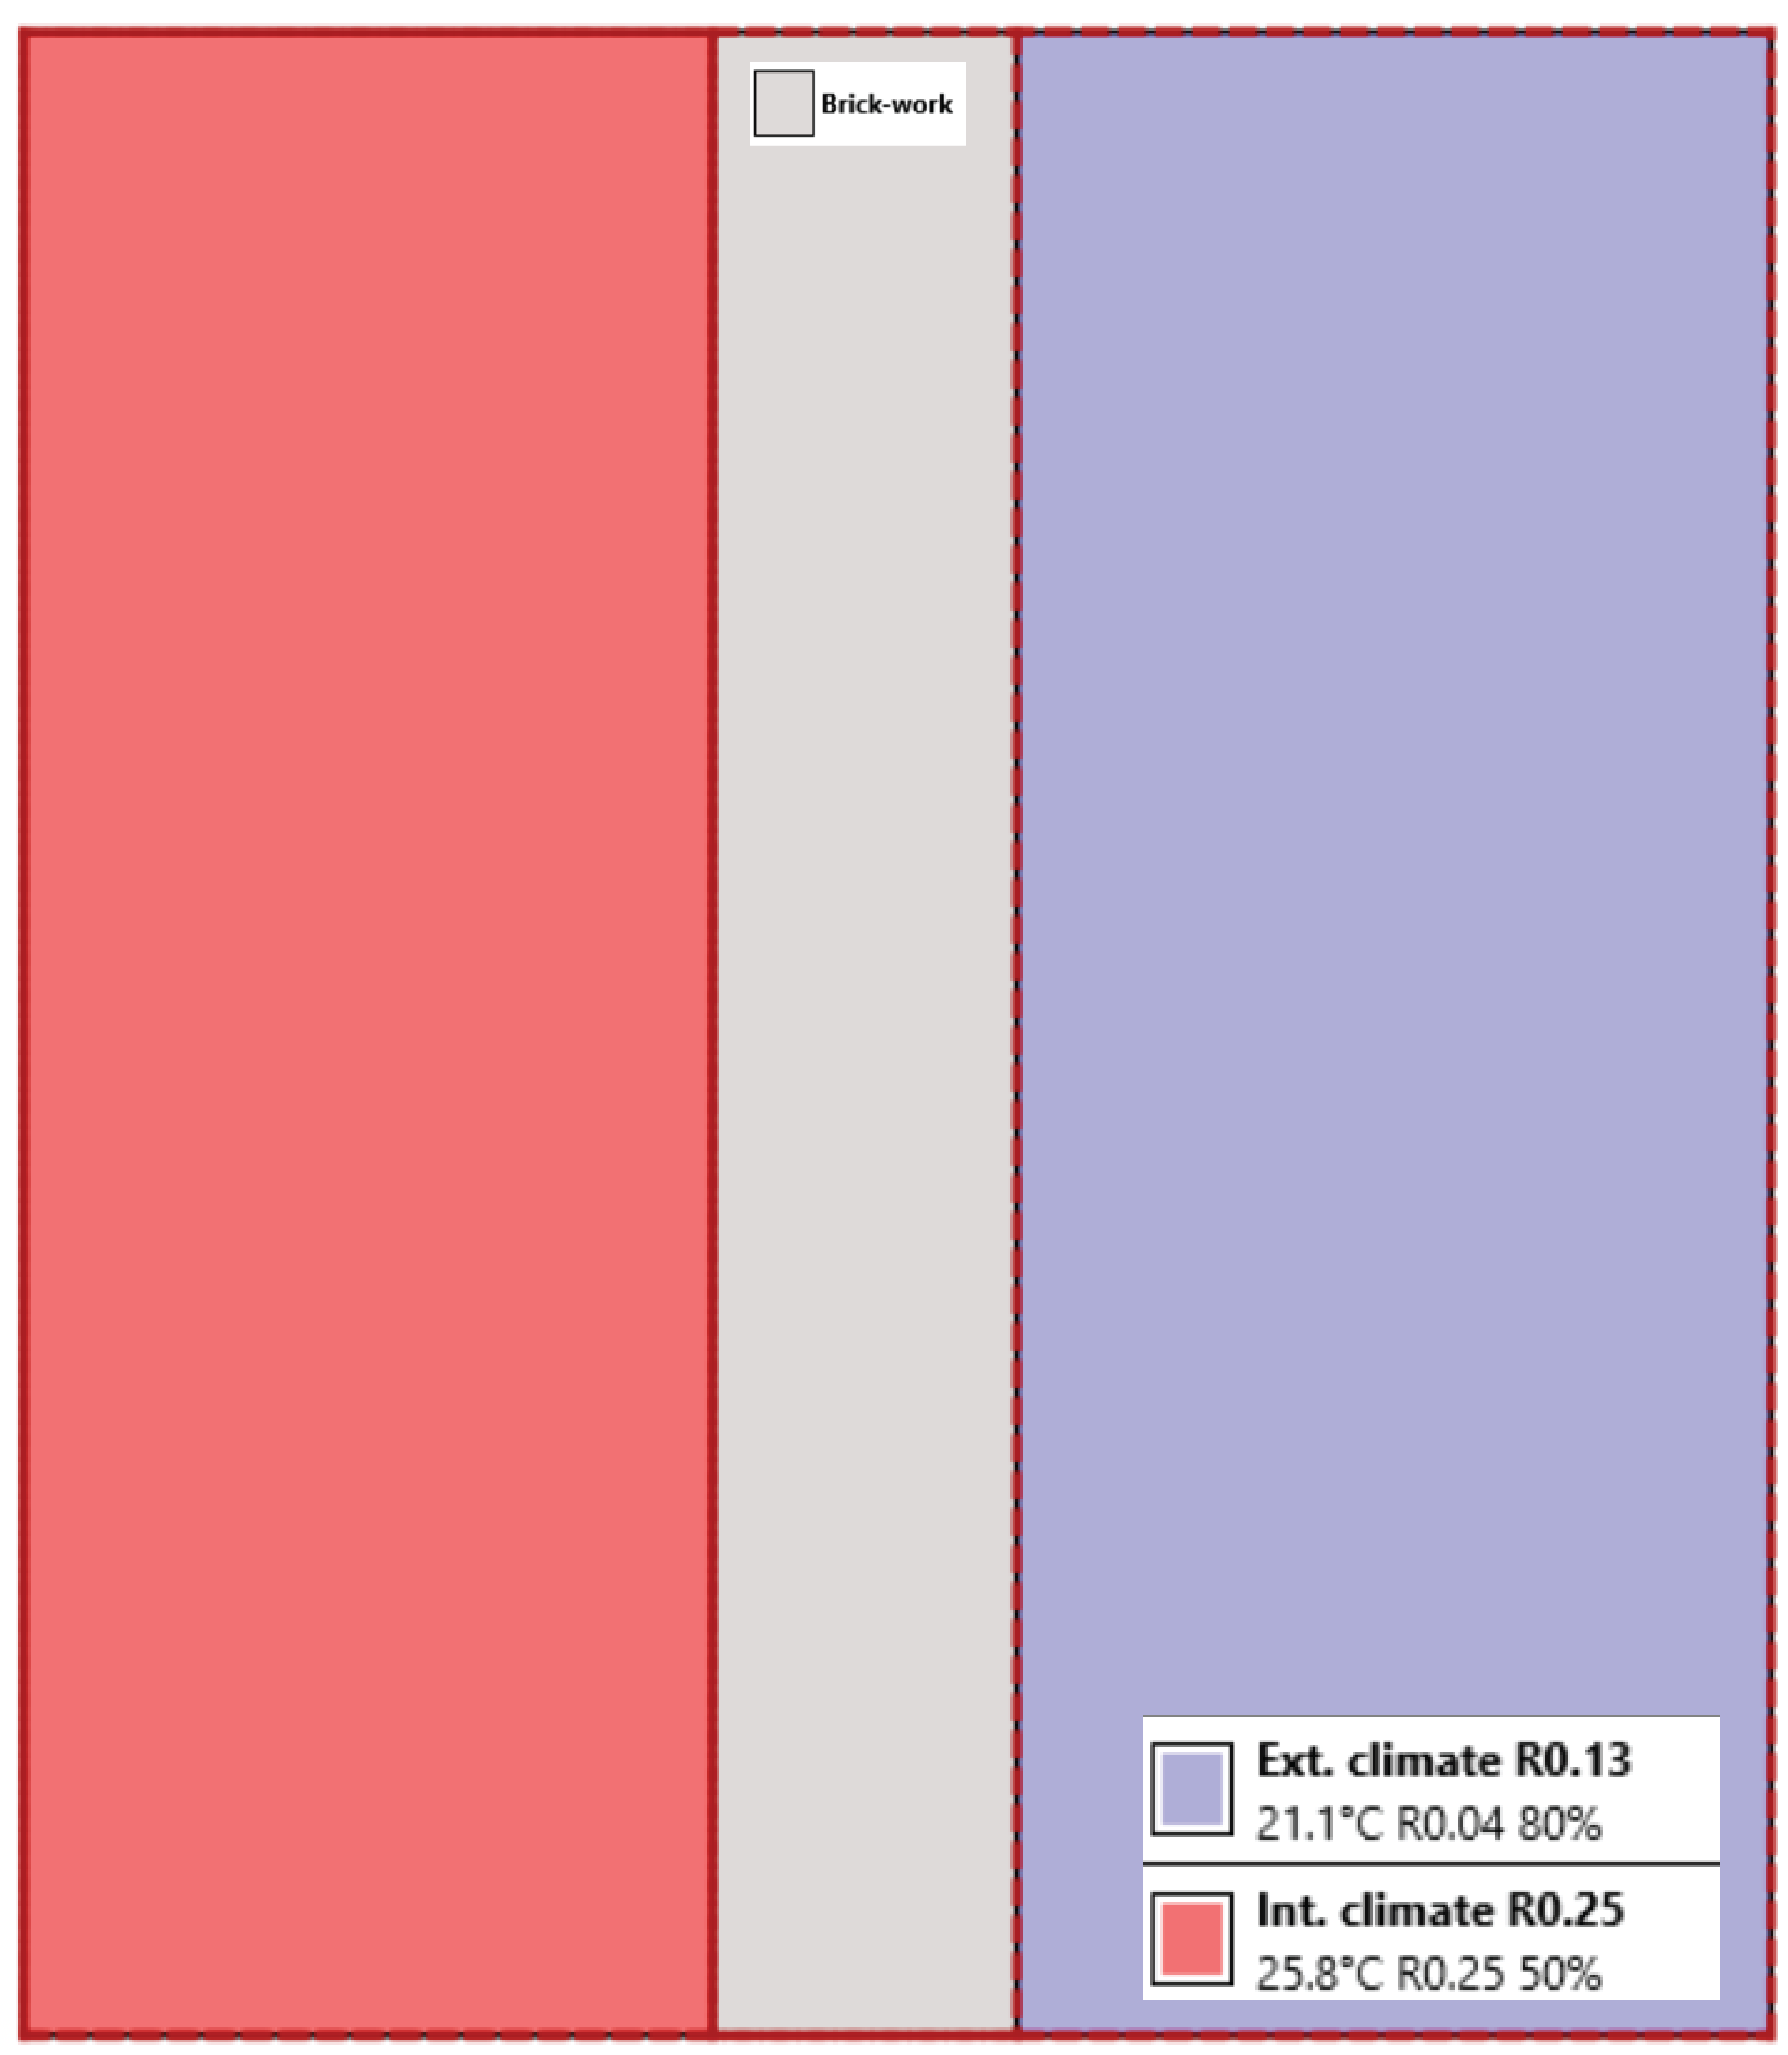
\includegraphics[width=\linewidth]{Figures/2dconst.png} 
  \caption*{\textbf{(a)} The simulation boundary conditions from HTFlux}
\end{minipage}%
\hspace{0.1\textwidth}
\begin{minipage}{0.45\textwidth}
  \centering
  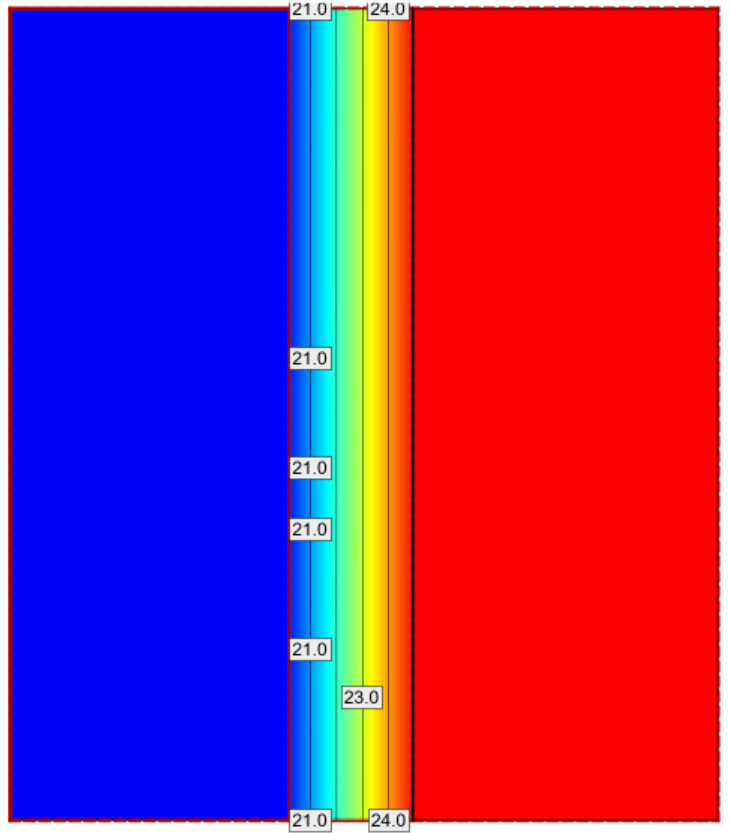
\includegraphics[width=\linewidth]{Figures/2dsim.png} 
  \caption*{\textbf{(b)} The brick wall temperature gradient results from HTFlux}
\end{minipage}
\caption{2D HTFlux Boundary conditions and Resulting heat flux of \( 10.91 \, {W/m}^2 \)}
\label{2dconst}
\end{figure}


\subsubsection{3D Simulation Compliance}\label{3dbrick}
Although chapter 4 explains the process of building the 3D heat transfer workflow in detail and validating the results with an ISO case, we returned to the brick wall in this chapter to model it with the 3D \gls{OF} simulation to further validate the results. So, the line plots in \ref{fig:expr} are the experimental design results and the points are the 3D heat transfer simulation results. \ref{error2d} is a comparison of the percentage of error between the results of the experiment and the 3D heat transfer workflow, where the average is from \%0.003 to \%0.01 and according to ISO\cite{ISO} to validate the case, the percentage of error shall not exceed \%0.1.


\begin{table}[H]
 \caption[2D Results Percentage error]{Percentage error demonstrating compliance between the experimental design results and the 3D workflow (in chapter 4) by calculating the percentage of error using the average method and the standard deviation method.}
    \label{error2d}
     \centering
 \begin{tabular}{l l l}
        \toprule
        Metric & T1 Percentage Error & T2 Percentage Error \\
        \midrule
        Average & 0.0032\% & 0.0102\% \\
        Standard Deviation & 0.0033\% & 0.0176\% \\
        \bottomrule
    \end{tabular}
\end{table}

\section{Discussion}
This section successfully presented the resources to calculate the heat flux of a 2D brick wall using three methods, which are by calculation, using sensors, using 2D simulation software where the heat flux q, respectively, = \( 10.93 \, {W/m}^2 \), \( 10.93 \, {W/m}^2 \), and \( 10.91 \, {W/m}^2 \). However, each of the presented approaches in this chapter are not convenient for an architect or a designer trying to seamlessly simulate 3D heat transfer. Thus, the gap of 3D heat transfer simulation integrated into the architecture modeling software is still missing and will be presented in the next chapter. In this chapter, \ref{3dbrick} is a work done after validating the 3D heat transfer tool, where the simulation is used to further validate the simulation using the brick wall example.